\section{Representations}
Goal of learning is to minimize the expected classification error, while maximizing generalization (avoid overfitting!).
We can't really do this. But we can minimize the \textit{empirical classification error} and maximize the \textit{estimated empirical generalization performance} by cross validation.

\subsection{The learning Problem}
\begin{itemize}
	\item Find function $f : \mathcal{X} \rightarrow \mathcal{Y}$ 
	\item Loss function $Q$ measures the deviation between $y$ and $f(x)$
	\begin{itemize}
		\item $(y-f(x))^2$ \quad  quadratic loss (regression)
		\item $\mathbb{I}_{\{y\neq f(x)\}}$ \quad 0-1 loss (classification)
		\item $\exp{(-\beta yf(x))}$ \quad  exponential loss (classification)
	\end{itemize}
	\item Conditional expected risk: \\$R(f,X) = \int_\mathcal{Y} Q(Y, f(X))P(Y|X)dY$
	\item Total Expected Risk: 
	\begin{multline*}
		R(f) = \mathbb{E}_X\left[R(f,X)\right]  = \int_\mathcal{X} R(f, X)P(X)dY\\ 
		= \int_\mathcal{Y} \int_\mathcal{X} Q(Y, f(X))P(X, Y)dXdY
	\end{multline*}
\end{itemize}

We divide the data intro training and test data to make sure we don't use the test data for calidation.
\begin{itemize}
	\item Empirical Risk Minimizer $\hat f \in \arg \min \hat R(f, \mathcal{Z}^{\text{train}})$ 
	\item Training Error: $\hat R(\hat f, \mathcal{Z}^\text{train}) = \frac{1}{n}\sum_{i=1}^n Q(Y_i, \hat f(X_i))$ 
	\item Test Error: $\hat R(\hat f, \mathcal{Z}^\text{test}) = \frac{1}{m}\sum_{i=n+1}^{n+m} Q(Y_i, \hat f(X_i))$
\end{itemize}

\subsubsection{Typical Approach}
\begin{enumerate}
	\item Feature Extraction (transform raw data to reduce information)
	\item Classifier Design
	\item Post-processing of classification results (adapt classifier output to enable stable scoring)
	\item Scoring
\end{enumerate}

\subsection{Taxonomy of Data}
Pattern Analysis = Find structure in sets of object representations.

\begin{itemize}
	\item Object Space $\mathcal{O}$
	\item Measurement mapping $x$ into a domain $\mathbb{K}$
\end{itemize}

\subsubsection{Data}
\begin{itemize}
	\item Monadic data: $X \to \mathbb R^d, o\mapsto X_o$ (water depth, temperature, pressure, intensity, ...)
	\item dyadic data $\mathcal O^{(1)} \times \mathcal O^{(1)} \to \mathbb R, (o_1, o_2) \mapsto X_{o_1, o_2}$ (e.g. (Users, Websites)). \\
		Pairwise Data: $\mathcal O \times \mathcal O \to \mathbb R, (o_1, o_2) \mapsto X_{o_1, o_2}$ (e.g. image patches x image patches)
	\item polyadic data
	\item ...
\end{itemize}
\begin{center}
	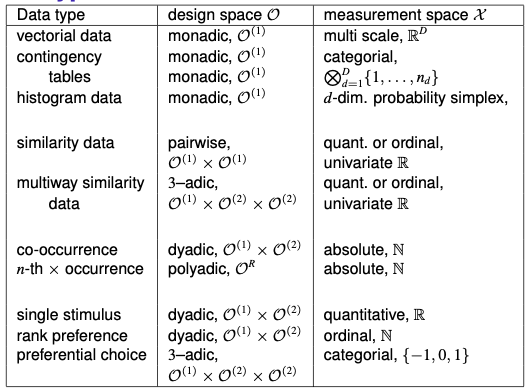
\includegraphics[width=0.8\columnwidth]{images/2-datatypes}
\end{center}

\subsection{Scales}
\begin{itemize}
	\item Nominal / Categorical: qualitattive, but without quantitative measurements (e.g. categories, binary, ...)
	\item Ordinal Scale: Values only meaningful w.r.t other measurements (rank order carries information, not the numerical differences)
	\item Quantitative Scale:
	\begin{itemize}
		\item Interval scale: relation of numerical differences carries the information
		\item Ratio scale: zero value of the scale carries information, but not the measurement unit
		\item Absolute scale: Absolute value is meaningful
	\end{itemize}
\end{itemize}

\subsection{Learning Pipeline: }
\begin{center}
	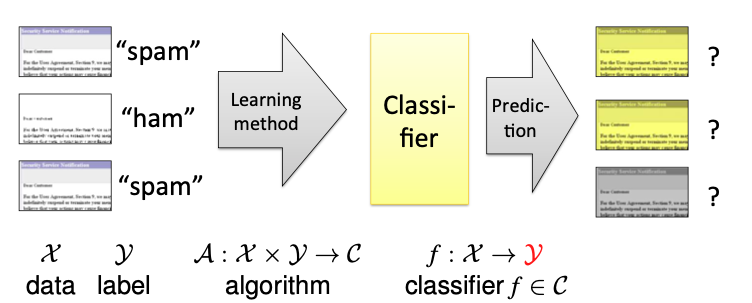
\includegraphics[width = 0.8\columnwidth]{images/2-pipeline}
\end{center}

\subsection{Mathematical Spaces}
A pair of objects $(\mathcal X, d)$ consisting of a non-empty set $\mathcal X$ and a function $d:\mathcal X \times \mathcal X \to \mathbb R$ is called a \textbf{metric space}, if:
\begin{enumerate}
	\item Positivity: $d(x,y) \geq 0 \forall x,y \in \mathcal X$
	\item Uniqueness $d(x,y) = 0 \iff x = y$
	\item Symmetry $d(x,y) = d(y,x)$
	\item $\triangle$-inequality: $d(x,z) \leq d(x,y) + d(y,z), x,y,z\in \mathcal X$
\end{enumerate}

\subsubsection{Euclidean Vector Space}
Let $\mathcal V = (\mathcal X, +, \cdot)$ a vector space. $x,y \in \mathcal V$. $\phi:\mathcal X \times \mathcal X \to \mathbb R$ is called \textbf{scalar product} if:
\begin{enumerate}
	\item Distributivity: $\phi(x_1. + x_2, y) = \phi(x_1, y) + \phi(x_2, y)$
	\item Commutativity: $\phi(x,y) = \phi(y,x)$
	\item Homogeneity: $\phi(\alpha x, y) = \alpha\phi(x,y)$
	\item Positive Definiteness: $\phi(x,x) > 0 \quad \forall x \neq 0$
\end{enumerate} 
A vector space with a scalar product is called \textbf{euclidean vector space}.

\subsubsection{Probability Spaces}
\begin{itemize}
	\item Elementary event: $\omega_1, ...k, \omega_N$ are sample points
	\item Sample space: $\Omega = \{\omega_1, ..., \omega_N\}$
	\item Family of Sets: Event $A$ of an experiment is a set of elementary events with $A \subset \Omega$, result of experiment is $\omega \in A$ or $\omega \not\in A$
	\item Algebra of events $\mathcal A$ = set of subsets $A\subset \Omega$ with $\Omega \in \mathcal A$ and $(A\in \mathcal A \land B \in \mathcal A \implies A\cup B \in \mathcal A \land A \cap B\in \mathcal A \land A \backslash B \in \mathcal A)$
\end{itemize}
Assign weights to elementary events with $0\leq p(\omega_i) \leq 1$ and $\sum_ip(w_i) = 1$. The \textbf{Probability of an event} $A\in \mathcal A$ with $P(A) = \sum_{\{i:w_i\in A\}} p(w_i)$

A \textbf{probability model} is a triple $(\Omega, \mathcal A, P)$, with $\mathcal P = \{P(A) \mid A \in \mathcal A\}$

\sepline